% ---
% template desenvolvido inicialmente por (DC-LESI) Prof Alberto Simões
% modificado/melhorado por João Carlos Pinto (#20808) LESI-PL
% ---
\documentclass[a4paper,12pt,twoside]{book}
\usepackage{lesi/lesi}

\title{Projeto OSLER}
\author{João Carlos Pinto, 20808 \AND André Mandim, 21160 \AND Rui Alves, 15505 \AND Augusto Pereira, 21136}
\LESI
\regimePosLaboral         % ou \regimeDiurno
\date{\today}

%% Caso tenham mais que um orientador, colocar
%% \orientador{Nome professor \AND Nome professor}
\orientador{Nuno Feixa Rodrigues \AND Óscar Ribeiro}

%% comentar estas três linhas para projectos
% \empresa{Fuzzy Bit - Software Engineering}
% \enderecoEmpresa{Barcelos, Portugal}
% \supervisor{Eng. A. U. Thor}


% comentar se não for para usar glossários
\makeglossaries


% inicio do documento
\begin{document}
 
\newglossaryentry{lematizador}
{
	name=lematizador,
	description={Com semelhanças com o Stemmer, também reduz uma palavra ao seu lema, que corresponde ao verbo no infinitivo no caso dos verbos, e ao masculino singular, no caso de nomes ou adjetivos. }
}
 
\newglossaryentry{stemmer} 
{
	name=stemmer,
	description={Ferramenta capaz de reduzir uma palavra à sua raiz. Por exemplo, para a palavra ``correria'', a sua raiz seria ``corre''. }
}
 
\newglossaryentry{triagemmanchester}
{
	name=Triagem de Manchester,
	description={O Protocolo de Triagem de Manchester foi implementado em novembro de 1994, em Manchester, com o objetivo expresso de estabelecer um consenso entre médicos e enfermeiros do Serviço de Urgência, com vista à criação de normas de triagem baseadas na determinação do risco clínico. \citep{grupoportuguestriagem}}
}
 
 
\newacronym{ftp}{FTP}{File Transfer Protocol (Protocolo de Transferência de Ficheiros) }
  
\newacronym{http}{HTTP}{HyperText Transfer Protocol (Protocolo de Transferência de Hipertexto)}

\newacronym{tcp}{TCP}{Transmission Control Protocol}

\newacronym{uctxt}{UC}{Unidade Curricular}

\newacronym{ucstxt}{UC}{Unidades Curriculares}

\newacronym{ucpds}{PDS}{Projeto de Desenvolvimento de Software}

\newacronym{ucpw}{PW}{Programação Web}

\newacronym{ucams}{AMS}{Análise e Modelação de Software}

\newacronym{ucaad}{AAD}{Armazenamento e Acesso a Dados}

\newacronym{ucpes}{PES}{Projeto de Engenharia de Software}

\newacronym{softalm}{ALM}{Aplication Lifecycle Management}

\newacronym{softsolid}{SOLID}{SOLID stands for Single Responsibility Principle (SRP), Open closed Principle (OSP), Liskov substitution Principle (LSP), Interface Segregation Principle (ISP), and Dependency Inversion Principle (DIP)}


\frontmatter
\maketitle  % print the title

\begin{resumo}
De uma forma geral, o serviço de urgência é o que regista mais visitas do que os restantes serviços de uma instituição de prestação de cuidados de saúde primários. Normalmente a sobrecarga deste serviço provoca um aumento dos tempos de espera porque o corpo clínico é constituído por recursos humanos finitos. Este problema pode afetar negativamente a instituição. Uma das principais causas identificadas é a presença de um elevado número de pessoas com uma condição clínica de baixa gravidade, i.e. com uma classificação de acordo com a determinação do risco clínico conforme o protocolo de \gls{triagemmanchester}.  
  
O Projeto OSLER propõe-se a fornecer um sistema complementar de apoio ao diagnóstico envolvendo o utente no processo de recolha de informações adicionais que possam estar relacionadas com o episódio de urgência.  
  
O tema deste projeto tem como base inicial de trabalho uma Dissertação de Mestrado de Paulo Alexandre Gonçalves Pacheco na Universidade do Minho com o tema "Self-service Kiosk-based Anamnesis System for Emergency Departments". O documento fornecido como base de trabalho foi fornecido pelo Professor Nuno Feixa Rodrigues que também supervisionou a dissertação.  
\end{resumo}

% \begin{abstract}
% This is the translation of the previous text. It should say the exact same thing. Please do not use % directly Google Translator.
% \end{abstract}

%% Comment the following part if you are not acknowledging anybody
%\begin{agradecimentos}
%[A secção de agradecimentos é a parte pessoal do documento, e o único sítio onde o aluno pode escrever de forma menos formal, usando o tipo de linguagem que lhe parecer adequado para as pessoas a quem agradece.] 
%\end{agradecimentos}

\tableofcontents

\mainmatter

% introdução

\chapter{Introdução}
De uma forma geral, o serviço de urgência é o que regista mais visitas do que os restantes serviços de uma instituição de prestação de cuidados de saúde primários. Normalmente a sobrecarga deste serviço provoca um aumento dos tempos de espera porque o corpo clínico é constituído por recursos humanos finitos. Este problema pode afetar negativamente a instituição. Uma das principais causas identificadas é a presença de um elevado numero de pessoas com uma condição clínica de baixa gravidade, i.e. com uma classificação de acordo com a determinação do risco clínico conforme o protocolo de \gls{triagemmanchester}. \\


\section{Contexto}
Este projeto é desenvolvido no âmbito da \acrshort{uctxt} de \acrshort{ucpds}. Pretende-se materializar todos os conhecimentos obtidos em diversas \acrshort{ucstxt} (\acrshort{ucaad}, \acrshort{ucams} e \acrshort{ucpes}) do semestre passado. 




\section{Objetivos}
O objetivo deste trabalho é dedicar todo o tempo da aula na implementação de um sistema de software. O sistema terá que ser implementado numa arquitetura com um \textbf{Web front-end} e um \textbf{back-end}. \\

\begin{itemize}
	\item O front-end desenvolvido na \acrshort{uctxt} de \acrlong{ucpw};
	\item O back-end desenvolvido na \acrshort{uctxt} de \acrlong{ucpds};
	\item A integração entre o front-end e o back-end será realizada através da uma API (\textit{\textbf{RESTful HTTP Services}});
	\item A metodologia \textbf{Scrum} será utilizada para o planeamento do projeto;
	\item O software \acrshort{softalm} escolhido para apoio à gestão deste projeto foi a plataforma Azure DevOps;
	\item Além deste documento, toda a informação será atualizada em documento excel na plataforma de E-learning da \acrshort{uctxt} de \acrlong{ucpds};
	\item Utilização de sistema de controlo de versões. Foi escolhido o Git que está incluído no espaço do projeto na plataforma Azure DevOps;
	\item A planificação do projeto será feita em 4 milestones para apresentar em aula (Especificação, vAlfa, vBeta e vRTW - Ready to Web).
\end{itemize}



\section{Estrutura do documento}
Este documento agrupa toda a documentação produzida pelo grupo de trabalho em todas as fases do projeto. \\

\begin{enumerate}
	\item Identificação do problema;
	\item Milestone Análise de requisitos e modelação. Especificação dos requisitos funcionais e não funcionais do sistema, \textit{mockups}, backlog completo e planeamento inicial de \textit{sprints};
	\item Milestone vAlfa. Requisitos funcionais implementados. Testar automaticamente todas as funcionalidades. Documentação de especificação deve incluir todas as alterações;
	\item Milestone vBeta. Sistema completamente implementado e funcional. Integração de todos os componentes. Identificar e apresentar aspetos funcionais e não funcionais a melhorar no sistema;
	\item Milestone vRTW. Versão final pronta a entrar em produção. Preparação de material promocional; 
	\item Conclusão deste documento;
\end{enumerate}

\subsection*{\textbf{NOTA}:}

Cada um dos capítulos da lista anterior inclui ainda dados referentes a todas as reuniões do grupo de trabalho. A parte alfanumérica que identifica cada reunião corresponde a cada \textit{milestone} do projeto:
\begin{itemize}
	\item \textbf{MM} = Milestone Análise de requisitos e modelação;
	\item \textbf{MA} = Milestone vAlfa;
	\item \textbf{MB} = Milestone vBeta;
	\item \textbf{MR} = Milestone vRTW. 
\end{itemize}


\section{Equipa}

A composição do grupo de trabalho, nome do projeto, nome da equipa e cargos foi finalizada na primeira reunião (identificada como reunião MM01 transcrita no capítulo \ref{reuniaoMM01} na página \pageref{reuniaoMM01}).\\[4mm]

\noindent \textbf{Nome do projeto}\\[1mm]
\noindent \rule{\linewidth}{0.4pt}
\noindent Projeto OSLER \\[4mm]

\noindent \textbf{Nome da equipa}\\[1mm]
\noindent \rule{\linewidth}{0.4pt}
\noindent Fuzzy Bit - Software Engineering \\[4mm]

\noindent \textbf{Membros e cargos}\\[1mm]
\noindent \rule{\linewidth}{0.4pt}
\noindent João Carlos Marques Pinto (20808) \textbf{Product Owner} + Development team member\\[1mm]
\noindent André Carvalho Mandim (21160) \textbf{Scrum Master} + Development team member\\[1mm]
\noindent António Augusto Fernandes Simões Pereira (21136) Development team member \\[1mm]
\noindent (*)Maria do Rosário Dias Figueiredo da Silva (21138) Development team member \\[1mm]
\noindent Rui Manuel da Silva Alves (15505) Development team member \\[2mm]

\noindent (*) decidiu sair do grupo a meio do primeiro milestone. \\[4mm]




% identificação do problema

\chapter{Identificação do problema}

A gestão de um serviço de urgência é uma área das instituições de prestação de cuidados de saúde primários. \\ 
A sobrecarga deste serviço provoca um aumento dos tempos de espera porque o corpo clínico é constituído por recursos humanos finitos. Este problema pode afetar negativamente a instituição. \\ 
Uma das principais causas identificadas é a presença de um elevado número de pessoas com uma condição clínica de baixa gravidade, i.e. com uma classificação de acordo com a determinação do risco clínico conforme o protocolo de Protocolo Triagem Manchester \citep{Triagem2022}. 



\section{Proposta}
O Projeto OSLER propõe-se a fornecer um sistema complementar de apoio ao diagnóstico envolvendo o utente no processo de recolha de informações adicionais que possam estar relacionadas com o episódio de urgência.  



\subsection{Infraestrutura...}
\begin{itemize}
	\item A instituição fornece as informações à plataforma via RESTful HTTP Services. Inicia e consulta o processo com todas as informações atualizadas pelo utente e pelos serviços até o episódio de urgência ficar concluído;
	\item O ID do episódio de urgência é fornecido à plataforma juntamente com dados adicionais do utente (Nome, cor da triagem, data/hora de entrada, número de utente SNS);
	\item Todos os utilizadores do sistema podem aceder à plataforma num dispositivo com browser e com acesso Wi-Fi à rede da instituição.
\end{itemize}



\subsection{Desenvolvimento...}
\begin{itemize}
	\item A linguagem de programação \textbf{C\#} foi a escolhida para o desenvolvimento do back-end;
	\item Serão utilizados e aplicados os princípios \acrshort{softsolid} \citep{Naidu2021}.
\end{itemize}



\subsection{O sistema...}
\begin{itemize}
	\item Deve controlar o acesso inicial ao processo de cada utente;
	\item Deve considerar diferentes níveis de acesso para os diferentes tipos de utilizadores;
	\item Deve registar o ID do utilizador, data/hora em cada operação registada;
	\item Deve reter ocultando todas as informações apagadas e introduzidas pelos utilizadores na base de dados, só no final do processo é que se poderá fazer a limpeza desses dados. Os utilizadores com nível de acesso superior podem consultar e recuperar esses dados caso sejam necessários;
	\item Deve considerar os seguintes tipos de utilizadores (utente, acompanhante, triagem, enfermeiro, médico, sysadmin);
	\item Deve considerar um interface para diferentes idiomas para os utilizadores;
	\item Deve suportar a criação de diferentes questionários;
	\item Deve permitir atualização do local onde o utente se encontra durante todo o processo;
	\item No caso de o utente ter algum dispositivo de monitorização, o sistema deverá permitir a introdução de diversas leituras dos valores no intervalo de tempo indicado ou programado pelo técnico de saúde;
	\item Deve permitir que o acompanhante do utente preencha e/ou atualize as informações dos questionários;
	\item Deve permitir associar mais do que um episódio a mais do que um técnico de saúde;
	\item Deve permitir que qualquer um dos técnicos de saúde (com acesso,) possam atualizar e/ou acrescentar valores no processo do utente;
	\item Deve permitir que um médico possa consultar episódios anteriores do utente, fazendo a pesquisa pelo número de SNS;
	\item Deve manter o episódio com estado ativo até ser dada alta ao utente, neste caso o estado será "fechado";
	\item Deve registar todas as deslocações e locais de espera, utilizando uma ordem sequencial onde deve ser incluída data/hora;
	\item Deve registar data/hora para cada resposta do questionário;
\end{itemize}



\subsection{Controlo de acesso dos utilizadores}
\begin{itemize}
	\item Os utilizadores dos diversos serviços são adicionados pelo sysadmin;
	\item Qualquer um dos utilizadores autorizados de cada serviço pode consultar um episódio com o estado "aberto";
	\item A autenticação do utente e do acompanhante é feita utilizando o nº do episódio e um PIN para o acesso inicial, depois o controlo da sessão é feito internamente utilizando um token;
	\item Internamente o utente/acompanhante é identificado no sistema pelo ID do episódio de urgência. O ID de utilizador nos registos será calculado automaticamente utilizando um dígito "0"(zero) para o utente e "1"(um) para o acompanhante respetivamente;
\end{itemize}





% Milestone Análise de requisitos e modelação

\chapter{Milestone Análise de requisitos e modelação}


% requisitos

\section{Requisitos}

\noindent Resultado da análise feita durante a reunião MM02 transcrita no capítulo \ref{reuniaoMM02} na página \pageref{reuniaoMM02}. \\

\noindent\textbf{Requisitos Funcionais} \\[4mm]
\begin{minipage}{\linewidth}
\begin{itemize}
	\item Para aceder ao sistema é obrigatório a autenticação por qualquer utilizador;
	\item Apenas o utilizador da triagem pode emitir episódios;
	\item O utente e o acompanhante podem responder a questionários;
	\item O acompanhante, enfermeiro e o medico podem visualizar os dados do utente;
	\item O utente e o acompanhante podem verificar qual a localização deveriam estar (sala/espaço);
	\item O acompanhante pode verificar onde está qual a localização do utente;
	\item Todos os utilizadores podem ver os seus dados;
	\item Todos os utilizadores podem introduzir dados métricos.
\end{itemize}
\end{minipage}
\newline

\noindent\textbf{Requisitos Não Funcionais} \\[4mm]
\begin{minipage}{\linewidth}
\begin{itemize}
	\item O sistema deverá ser compatível com sistema Windows, OSX, Android e iOS;
	\item O design do sistema deverá ser compatível com HTML5;
	\item O sistema deverá conter uma proteção por password;
	\item As conexões deverão estar protegidas por Tokens.
\end{itemize}
\end{minipage}
\newline

% Diagrama: Casos de Uso

\section{Diagrama: Casos de Uso}

Atores identificados (Triagem, Utente, Acompanhante, Enfermeiro, Médico, Sysadmin)
\newline

\subsection{CdU1 Triagem}

\begin{minipage}{\linewidth}
\begin{itemize}
	\item \textbf{CdU1.1}: Como Triagem tenho a possibilidade de autenticar (figura~\ref{fig:cdu3111});
	\item \textbf{CdU1.2}: Como Triagem tenho a possibilidade de emitir episódios (figura~\ref{fig:cdu3111}).
\end{itemize}
\end{minipage}
\newline
  
\subsection{CdU2 Utente}

\begin{minipage}{\linewidth}
\begin{itemize}
	\item \textbf{CdU2.1}: Como Utente tenho a possibilidade de autenticar (figura~\ref{fig:cdu3112});
	\item \textbf{CdU2.2}: Como Utente tenho a possibilidade de responder a questionários (figura~\ref{fig:cdu3113});
	\item \textbf{CdU2.3}: Como Utente tenho a possibilidade de ter acesso ao meus dados (figura~\ref{fig:cdu3112});
	\item \textbf{CdU2.4}: Como Utente tenho a possibilidade de ter acesso à localização (sala onde tenho de estar e para onde terei de ir) (figura~\ref{fig:cdu3113});
	\item \textbf{CdU2.5}: Como Utente tenho a possibilidade de introduzir dados métricos (figura~\ref{fig:cdu3112});
	\item \textbf{CdU2.6}: Como Utente tenho a possibilidade de alterar as respostas dos questionários (figura~\ref{fig:cdu3113}).
\end{itemize}
\end{minipage}
\newline

\subsection{CdU3 Acompanhante}
\begin{minipage}{\linewidth}
\begin{itemize}
	\item \textbf{CdU3.1}: Como Acompanhante tenho a possibilidade de autenticar (figura~\ref{fig:cdu3112});
	\item \textbf{CdU3.2}: Como Acompanhante tenho a possibilidade de responder a questionários relativamente a mim e ao utente que estou a acompanhar (figura~\ref{fig:cdu3110});
	\item \textbf{CdU3.3}: Como Acompanhante tenho a possibilidade de ter acesso aos dados do utente que estou a acompanhar (figura~\ref{fig:cdu3110});
	\item \textbf{CdU3.4}: Como Acompanhante tenho a possibilidade de ter acesso à localização do utente que estou a acompanhar (sala onde tenho de estar e para onde terei de ir) (figura~\ref{fig:cdu3110});
	\item \textbf{CdU3.5}: Como Acompanhante tenho a possibilidade de introduzir dados métricos do utente que estou a acompanhar (figura~\ref{fig:cdu3110}).
\end{itemize}
\end{minipage}
\newline

\subsection{CdU4 Enfermeiro}
\begin{minipage}{\linewidth}
\begin{itemize}
	\item \textbf{CdU4.1}: Como Enfermeiro tenho a possibilidade de autenticar (figura~\ref{fig:cdu3112});
	\item \textbf{CdU4.2}: Como Enfermeiro tenho a possibilidade de visualizar os dados dos utentes (figura~\ref{fig:cdu3112});
	\item \textbf{CdU4.3}: Como Enfermeiro tenho a possibilidade de introduzir dados métricos (figura~\ref{fig:cdu3112}).
\end{itemize}
\end{minipage}
\newline

\subsection{CdU5 Médico}
\begin{minipage}{\linewidth}
\begin{itemize}
	\item \textbf{CdU5.1}: Como Médico tenho a possibilidade de autenticar (figura~\ref{fig:cdu3112});
	\item \textbf{CdU5.2}: Como Médico tenho a possibilidade de visualizar os dados dos utentes (figura~\ref{fig:cdu3112});
	\item \textbf{CdU5.3}: Como Médico tenho a possibilidade de introduzir dados métricos (figura~\ref{fig:cdu3112});
	\item \textbf{CdU5.4}: Como Médico tenho a possibilidade de alterar o local do utente (figura~\ref{fig:cdu3112});
	\item \textbf{CdU5.5}: Como Médico tenho a possibilidade de alterar o estado do episódio (figura~\ref{fig:cdu3112});
	\item \textbf{CdU5.6}: Como Médico tenho a possibilidade de verificar o histórico de um utente (figura~\ref{fig:cdu3112}).
\end{itemize}
\end{minipage}
\newline

\subsection{CdU6 Sysadmin}
\begin{minipage}{\linewidth}
\begin{itemize}
	\item \textbf{CdU6.1}: Como Sysadmin tenho a possibilidade de autenticar (figura~\ref{fig:cdu3113});
	\item \textbf{CdU6.2}: Como Sysadmin tenho a possibilidade de criar questionários (figura~\ref{fig:cdu3113});
	\item \textbf{CdU6.3}: Como Sysadmin tenho a possibilidade de adicionar idiomas (figura~\ref{fig:cdu3113});
	\item \textbf{CdU6.4}: Como Sysadmin tenho a possibilidade de adicionar locais (figura~\ref{fig:cdu3113});
	\item \textbf{CdU6.5}: Como Sysadmin tenho a possibilidade de adicionar dados métricos reconhecíveis do sistema (figura~\ref{fig:cdu3113});
	\item \textbf{CdU6.6}: Como Sysadmin tenho a possibilidade de adicionar, editar, desativar utilizadores (figura~\ref{fig:cdu3113}).
\end{itemize}
\end{minipage}
\newline

As imagens dos diagramas de casos de uso apresentados no documento são referenciados em cada um dos Casos de Uso.

\begin{figure}[htbp]
	\centering
	\includegraphics[width=0.5\linewidth]{img/Utente\_v0.png}  % largura percentual 
	\caption{CdU exclusivo do Utente e Acompanhante}
	\label{fig:cdu3110}
\end{figure}


\begin{figure}[htbp]
	\centering
	\includegraphics[width=0.5\linewidth]{img/CdU1\_v1.png}  % largura percentual 
	\caption{CdU comum a diversos atores (parte1)}
	\label{fig:cdu3111}
\end{figure}


\begin{figure}[htbp]
	\centering
	\includegraphics[width=0.5\linewidth]{img/UseCase\_v2.png}  % largura percentual 
	\caption{CdU comum a diversos atores (parte2)}
	\label{fig:cdu3112}
\end{figure}


\begin{figure}[htbp]
	\centering
	\includegraphics[width=0.5\linewidth]{img/Sysadmin\_v1.png}  % largura percentual 
	\caption{CdU exclusivo do Sysadmin}
	\label{fig:cdu3113}
\end{figure}



% Diagrama: Component Diagram

\section{Diagrama: Component Diagram}
A imagem identificada neste documento como figura~\ref{fig:cd3120} representa a versão inicial do diagrama de componentes.

\begin{figure}[htb]
	\centering
	\includegraphics[width=0.9\linewidth]{img/Component\_Diagram\_v0.png}  % largura percentual 
	\caption{Component Diagram}
	\label{fig:cd3120}
\end{figure}


% Diagrama: Class Diagram

\section{Diagrama: Class Diagram}\label{oldClasseDiagram}

A imagem identificada neste documento como figura~\ref{fig:cd3130} representa a versão base simplificada do diagrama de classes. 

\noindent NOTA: Este diagrama foi ampliado e melhorado na \textbf{Milestone vAlfa}. Todas as informações encontram-se na página ~\pageref{novoClasseDiagram} na secção \ref{novoClasseDiagram} deste documento.

\begin{figure}[htb]
	\centering
	\includegraphics[width=0.9\linewidth]{img/Class\_Diagram\_v4\_v0\_base.png}  % largura percentual 
	\caption{Class Diagram (versão base simplificada)}
	\label{fig:cd3130}
\end{figure}



% Diagrama: Interaction Overview Diagram

\section{Diagrama: Interaction Overview Diagram}
\begin{minipage}{\linewidth}
A imagem identificada neste documento como figura~\ref{fig:iod3140} representa a versão inicial do diagrama de visão geral da interação. A operação apresentada graficamente simula a consulta de informações do Utente feita pelo Médico.
\end{minipage}

\begin{figure}[htb]
	\centering
	\includegraphics[width=0.9\linewidth]{img/Interaction\_Diagram\_medico\_v0.png}  % largura percentual 
	\caption{Interaction Overview Diagram}
	\label{fig:iod3140}
\end{figure}


% Diagrama: Activity Diagram

\section{Diagrama: Activity Diagram}

\begin{minipage}{\linewidth}
Escolhemos os seguintes cenários para o diagrama de atividade.
\begin{itemize}
	\item Processo de triagem (figura~\ref{fig:adg3150});
	\item Processo normal do utente (figura~\ref{fig:adg3150});
	\item Processo normal do médico (figura~\ref{fig:adg3150}).
\end{itemize}
\end{minipage}

\begin{figure}[htb]
	\centering
	\includegraphics[height=0.9\linewidth]{img/Activity\_diagram\_grupo\_v0.png}  % largura percentual 
	\caption{Diagrama de atividade}
	\label{fig:adg3150}
\end{figure}


% Diagrama: Sequence Diagram

\section{Diagrama: Sequence Diagram}
A imagem identificada neste documento como figura~\ref{fig:sd3160} representa a versão inicial do diagrama de sequência.

\begin{figure}[htb]
	\centering
	\includegraphics[width=0.9\linewidth]{img/Sequence\_diagram\_utente\_v0.png}  % largura percentual 
	\caption{Sequence Diagram}
	\label{fig:sd3160}
\end{figure}



% Diagrama: Entity-Relationship Diagram

\section{Diagrama: Entity-Relationship Diagram}
A imagem identificada neste documento como figura~\ref{fig:erd3170} representa a versão inicial do diagrama ER.

\begin{figure}[htb]
	\centering
	\includegraphics[width=0.9\linewidth]{img/ER\_Diagram\_v1\_v2.png}  % largura percentual 
	\caption{Entity-Relationship Diagram}
	\label{fig:erd3170}
\end{figure}



% Backlog

\section{Backlog}


\subsection{Features}

\begin{minipage}{\linewidth}
\begin{itemize}
	\item O sistema será capaz de permitir aos utilizadores registar dados métricos, e aos que assim for designado consultá-los;
	\item O sistema será capaz de permitir aos utentes e aos acompanhantes responder a questionários e facultar as respostas aos médicos;
	\item O sistema será capaz de permitir que os utentes e acompanhantes tenham acesso à localização atual e esperada(futura) do utente. 
\end{itemize}
\end{minipage}


\subsection{Backlog items}
A imagem identificada neste documento como figura~\ref{fig:pb3180} representa a versão inicial do product backlog do projeto.

\begin{figure}[htb]
	\centering
	\includegraphics[width=0.9\linewidth]{img/Product\_backlog\_v3.png}  % largura percentual 
	\caption{Product Backlog}
	\label{fig:pb3180}
\end{figure}


\subsection{Tasks}

\begin{minipage}{\linewidth}
\begin{itemize}
	\item Tasks Sprint1 Milestone Análise de requisitos e modelação (figura~\ref{fig:task3181});
\end{itemize}
\end{minipage}

\begin{figure}[htb]
	\centering
	\includegraphics[width=0.9\linewidth]{img/milestone\_analise\_sprint1\_v2.png}  % largura percentual 
	\caption{Tasks Sprint1 Milestone Análise de requisitos e modelação}
	\label{fig:task3181}
\end{figure}


% Mockups

\section{Mockups}

No processo de análise identificamos o layout das seguintes operações:

\begin{minipage}{\linewidth}
	Perfil geral:
\begin{itemize}
	\item Janela de autenticação (figura~\ref{fig:mckg01});
\end{itemize}
\end{minipage}

\begin{minipage}{\linewidth}
	Perfil do médico:
\begin{itemize}
	\item Página de consulta do utente (figura~\ref{fig:mckm01});
	\item Página de consulta do episódio (figura~\ref{fig:mckm02});
\end{itemize}
\end{minipage}

\begin{minipage}{\linewidth}
	Perfil da triagem:
\begin{itemize}
	\item Página de criação de episódio (figura~\ref{fig:mckt01});
\end{itemize}
\end{minipage}

\begin{minipage}{\linewidth}
	Perfil do utente:
\begin{itemize}
	\item Página de consulta de episódio (figura~\ref{fig:mcku01});
	\item Página de consulta de dados pessoais (figura~\ref{fig:mcku02});
	\item Página de resposta de questionário (figura~\ref{fig:mcku03}).
\end{itemize}
\end{minipage}

\begin{minipage}{\linewidth}
	Perfil do sysadmin:
	\begin{itemize}
		\item Página de consulta do utilizador (figura~\ref{fig:mcks01});
		\item Página de consulta do questionário (figura~\ref{fig:mcks02});
	\end{itemize}
\end{minipage}

% imagens do perfil geral
\begin{figure}[htb]
	\centering
	\includegraphics[width=0.5\linewidth]{img/Mockups\_login\_v1.png}  % largura percentual 
	\caption{Mockup - página de autenticação}
	\label{fig:mckg01}
\end{figure}

% imagens do perfil do médico
\begin{figure}[htb]
	\centering
	\includegraphics[width=0.5\linewidth]{img/Mockups\_medico\_consultautente\_v1.png}  % largura percentual 
	\caption{Mockup - Médico - página consulta utente}
	\label{fig:mckm01}
\end{figure}

\begin{figure}[htb]
	\centering
	\includegraphics[width=0.5\linewidth]{img/Mockups\_medico\_episodio\_v0.png}  % largura percentual 
	\caption{Mockup - Médico - página consulta episódio}
	\label{fig:mckm02}
\end{figure}

% imagens do perfil da triagem
\begin{figure}[htb]
	\centering
	\includegraphics[width=0.5\linewidth]{img/Mockups\_triagem\_novoepisodio\_v1.png}  % largura percentual 
	\caption{Mockup - Triagem - página criar episódio}
	\label{fig:mckt01}
\end{figure}

% imagens do perfil do utente
\begin{figure}[htb]
	\centering
	\includegraphics[width=0.5\linewidth]{img/Mockups\_utente\_infoepisodio\_v1.png}  % largura percentual 
	\caption{Mockup - Utente - página consultar episódio}
	\label{fig:mcku01}
\end{figure}

\begin{figure}[htb]
	\centering
	\includegraphics[width=0.5\linewidth]{img/Mockups\_utente\_dadospessoais\_v1.png}  % largura percentual 
	\caption{Mockup - Utente - página consultar dados pessoais}
	\label{fig:mcku02}
\end{figure}

\begin{figure}[htb]
	\centering
	\includegraphics[width=0.5\linewidth]{img/Mockups\_utente\_questionario\_v1.png}  % largura percentual 
	\caption{Mockup - Utente - página responder questionário}
	\label{fig:mcku03}
\end{figure}

% imagens do perfil do sysadmin
\begin{figure}[htb]
	\centering
	\includegraphics[width=0.5\linewidth]{img/Mockups\_sysadmin\_utilizador\_v0.png}  % largura percentual 
	\caption{Mockup - Sysadmin - página do utilizador}
	\label{fig:mcks01}
\end{figure}

\begin{figure}[htb]
	\centering
	\includegraphics[width=0.5\linewidth]{img/Mockups\_sysadmin\_questionario\_v0.png}  % largura percentual 
	\caption{Mockup - Sysadmin - página do questionário}
	\label{fig:mcks02}
\end{figure}


% Planeamento de sprints

\section{Planeamento de \textit{sprints}}

Data das \textit{sprints} de cada \textit{milestone} conforme decidido na reunião MM03 transcrita no capítulo \ref{reuniaoMM03} na página \pageref{reuniaoMM03}.\\[4mm]

\begin{minipage}{\linewidth}
\noindent \textbf{Especificação}\\[1mm]
\noindent \rule{\linewidth}{0.4pt}
\noindent \textbf{Sprint \#1}\\[1mm]
\noindent 03 março : data da sprint planning meeting\\[1mm]
\noindent 15 março : data da sprint review\\[4mm]
\end{minipage}

\begin{minipage}{\linewidth}
\noindent \textbf{Release Alpha}\\[1mm]
\noindent \rule{\linewidth}{0.4pt}
\noindent \textbf{Sprint \#1}\\[1mm]
\noindent 16 março : data da sprint planning meeting\\[1mm]
\noindent 23 março : data da sprint review\\[3mm]
\noindent \textbf{Sprint \#2}\\[1mm]
\noindent 24 março : data da sprint planning meeting\\[1mm]
\noindent 30 março : data da sprint review\\[3mm]
\noindent \textbf{Sprint \#3}\\[1mm]
\noindent 31 março : data da sprint planning meeting\\[1mm]
\noindent 06 abril : data da sprint review\\[3mm]
\end{minipage}

\begin{minipage}{\linewidth}
\noindent \textbf{Sprint \#4}\\[1mm]
\noindent 07 abril : data da sprint planning meeting\\[1mm]
\noindent 13 abril : data da sprint review\\[3mm]
\noindent \textbf{Sprint \#5}\\[1mm]
\noindent 14 abril : data da sprint planning meeting\\[1mm]
\noindent 20 abril : data da sprint review\\[3mm]
\noindent \textbf{Sprint \#6}\\[1mm]
\noindent 21 abril : data da sprint planning meeting\\[1mm]
\noindent 27 abril : data da sprint review\\[4mm]
\end{minipage}

\begin{minipage}{\linewidth}
\noindent \textbf{Release Beta}\\[1mm]
\noindent \rule{\linewidth}{0.4pt}
\noindent \textbf{Sprint \#1}\\[1mm]
\noindent 28 abril : data da sprint planning meeting\\[1mm]
\noindent 04 maio : data da sprint review\\[3mm]
\noindent \textbf{Sprint \#2}\\[1mm]
\noindent 05 maio : data da sprint planning meeting\\[1mm]
\noindent 11 maio : data da sprint review\\[3mm]
\noindent \textbf{Sprint \#3}\\[1mm]
\noindent 12 maio : data da sprint planning meeting\\[1mm]
\noindent 18 maio : data da sprint review\\[4mm]
\end{minipage}

\begin{minipage}{\linewidth}
\noindent \textbf{Release to Web}\\[1mm]
\noindent \rule{\linewidth}{0.4pt}
\noindent \textbf{Sprint \#1}\\[1mm]
\noindent 19 maio : data da sprint planning meeting\\[1mm]
\noindent 25 maio : data da sprint review\\[3mm]
\noindent \textbf{Sprint \#2}\\[1mm]
\noindent 26 maio : data da sprint planning meeting\\[1mm]
\noindent 01 junho : data da sprint review\\[3mm]
\noindent \textbf{Sprint \#3} (* preparação apresentação)\\[1mm]
\noindent 05 junho : data da sprint planning meeting\\[1mm]
\noindent 07 junho : data da sprint review\\[4mm]
\end{minipage}



% reuniões

\chapter{Milestone Análise: Reuniões}



\section{Reunião MM01}\label{reuniaoMM01}

\subsection*{Data:}
03-março-2022

\subsection*{Intervenientes:}
Grupo de trabalho

\subsection*{Âmbito:}
Constituir a equipa, identificar um nome para o grupo e para o projeto e iniciar o processo de análise. \\

\subsection*{Descrição:}
\textbf{*} Reunir os membros do grupo e atribuir os cargos. \\
João Carlos Marques Pinto (20808) Product Owner + Development team member\\
André Carvalho Mandim (21160) Scrum Master + Development team member\\
António Augusto Fernandes Simões Pereira (21136) Development team member \\
(*)Maria do Rosário Dias Figueiredo da Silva (21138) Development team member \\
Rui Manuel da Silva Alves (15505) Development team member \\
\noindent (*) decidiu sair do grupo a meio do primeiro milestone. \\

\textbf{*} Atribuir um nome ao grupo de trabalho. \\
O nome "Fuzzy Bit" foi o que reuniu consenso. \\

\textbf{*} Atribuir um nome ao projeto. \\
"Projeto OSLER" foi o que reuniu consenso. \\

\textbf{*} Inicio do processo de análise do projeto: \\
Depois de diversas ideias terem sido lançadas no debate inicial, chegamos a um consenso sobre a ideia de funcionamento da aplicação no processo inicial:

\begin{itemize}
	\item Receção faz entrada(identificação);
	\item Vai a triagem (avaliação, responde a questões -> atribui uma prioridade);
	\item Sistema recolhe mais dados (questionários, registo de valores, monitorização do doente pelo acompanhante);
	\item Consulta (médico além das perguntas normais, tem acesso aos dados que o doente introduziu).
\end{itemize}

Algumas \textit{features} identificadas:
\begin{itemize}
	\item O utente(acompanhante/enfermeiro) fornece informação útil para a consulta (entre a triagem e a consulta com o médico);
	\item O acompanhante tem acesso à localização (sala de espera ou serviço) do doente.
\end{itemize}

\noindent \rule{\linewidth}{0.4pt}
\newline


\section{Reunião MM02}\label{reuniaoMM02}

\subsection*{Data:}
05-março-2022

\subsection*{Intervenientes:}
Grupo de trabalho

\subsection*{Âmbito:}
Discussão dos casos de uso.

\subsection*{Descrição:}
Definição dos requisitos funcionais e não funcionais.

\subsection*{Requisitos}

\textbf{Requisitos Funcionais}

\begin{itemize}
	\item O utilizador da triagem apenas pode emitir episódios;
	\item O utente e o acompanhante podem responder a questionários;
	\item O acompanhante, enfermeiro e o medico podem visualizar os dados do utente;
	\item O utente e o acompanhante podem verificar qual a localização deveriam estar (sala/espaço);
	\item O acompanhante pode verificar onde está qual a localização do utente;
	\item Todos os utilizadores podem ver os seus dados;
	\item Todos os utilizadores podem introduzir dados métricos.
\end{itemize}

\textbf{Requisitos Não Funcionais}

\begin{itemize}
	\item O sistema deverá ser compatível com sistema Windows, OSX, Android e iOS;
	\item O design do sistema deverá ser compatível com HTML5;
	\item O sistema deverá conter uma proteção por password;
	\item As conexões deverão estar protegidas por Tokens.
\end{itemize}

\noindent \rule{\linewidth}{0.4pt}
\newline


\section{Reunião MM03}\label{reuniaoMM03}

\subsection*{Data:}
07-março-2022

\subsection*{Intervenientes:}
Grupo de trabalho

\subsection*{Âmbito:}
Distribuição  dos sprints pelo tempo.

Definição das tarefas e algumas responsabilidades do primeiro sprint.

\subsection*{Descrição:}
Depois de alguma discussão foram definidas as seguintes datas:  \\[5mm]
\quad \textbf{Alpha inicio}\\[1mm]
\quad 16 março -> 22 março\\[1mm]
\quad 24 março -> 29 março\\[1mm]
\quad 31 março -> 05 abril\\[1mm]
\quad 07 abril -> 12 abril\\[1mm]
\quad 14 abril -> 19 abril\\[1mm]
\quad 21 abril -> 26 abril\\[1mm]
\quad \textbf{Alpha fim} \\[5mm]
\quad \textbf{Beta inicio}\\[1mm]
\quad 28 abril -> 03 maio\\[1mm]
\quad 05 maio -> 10 maio\\[1mm]
\quad 12 maio -> 17 maio\\[1mm]
\quad \textbf{Beta fim}\\[5mm]
\quad \textbf{rTW inicio}\\[1mm]
\quad 19 maio -> 24 maio\\[1mm]
\quad 26 maio -> 31 maio\\[1mm]
\quad 02 junho -> 07 de junho (preparar a apresentação) \\[1mm]
\quad \textbf{rTW fim} \\[5mm]

\noindent \rule{\linewidth}{0.4pt}
\newline

\section{Reunião MM04}\label{reuniaoMM04}

\subsection*{Data:}
16-março-2022

\subsection*{Intervenientes:}
Grupo de trabalho e professor

\subsection*{Âmbito:}
Sprint review.
Final da milestone de especificação.
Revisão do professor do trabalho feito.
Marcação das reuniões de acompanhamento do projeto.

\subsection*{Descrição:}

diagrama de classes - falta atributos e métodos

diagrama de atividades - explorar interação entre diferentes atores (usar com pools)

reuniões PDS:
\begin{itemize}
	\item23 março
	\item6 abril
	\item20 abril
	\item27 abril
	\item11 maio
	\item25 maio
\end{itemize}

\noindent \rule{\linewidth}{0.4pt}
\newline
 

% Milestone vAlfa

\chapter{Milestone vAlfa}



\subsection{Tasks vAlfa}

\begin{minipage}{\linewidth}
	\begin{itemize}
		\item Tasks Sprint1 - Milestone vAlfa (figura~\ref{fig:task4001}) em conformidade com a reunião MA01 transcrita no capítulo \ref{reuniaoMA01} na página \pageref{reuniaoMA01};
		\item Tasks Sprint2 - Milestone vAlfa (figura~\ref{fig:task4002}) em conformidade com a reunião MA03 transcrita no capítulo \ref{reuniaoMA03} na página \pageref{reuniaoMA03};
		\item Tasks Sprint3 - Milestone vAlfa (figura~\ref{fig:task4003}) em conformidade com a reunião MA05 transcrita no capítulo \ref{reuniaoMA05} na página \pageref{reuniaoMA05};
		\item Tasks Sprint4 - Milestone vAlfa (figura~\ref{fig:task4004}) em conformidade com a reunião MA07 transcrita no capítulo \ref{reuniaoMA07} na página \pageref{reuniaoMA07};
		\item Tasks Sprint5 - Milestone vAlfa (figura~\ref{fig:task4005}) em conformidade com a reunião MA09 transcrita no capítulo \ref{reuniaoMA09} na página \pageref{reuniaoMA09};
		\item Tasks Sprint6 - Milestone vAlfa (figura~\ref{fig:task4006}) em conformidade com a reunião MA11 transcrita no capítulo \ref{reuniaoMA11} na página \pageref{reuniaoMA11};
	\end{itemize}
\end{minipage}


\begin{figure}[htb]
	\centering
	\includegraphics[width=0.6\linewidth]{img/milestone\_vAlfa\_sprint1\_v2.png}  % largura percentual 
	\caption{Planeamento das tasks para a Sprint1 Milestone vAlfa}
	\label{fig:task4001}
\end{figure}


\begin{figure}[htb]
	\centering
	\includegraphics[width=0.6\linewidth]{img/milestone\_vAlfa\_sprint2\_v1.png}  % largura percentual 
	\caption{Planeamento das tasks para a Sprint2 Milestone vAlfa}
	\label{fig:task4002}
\end{figure}


\begin{figure}[htb]
	\centering
	\includegraphics[width=0.6\linewidth]{img/milestone\_vAlfa\_sprint3\_v1.png}  % largura percentual 
	\caption{Planeamento das tasks para a Sprint3 Milestone vAlfa}
	\label{fig:task4003}
\end{figure}


\begin{figure}[htb]
	\centering
	\includegraphics[width=0.6\linewidth]{img/milestone\_vAlfa\_sprint4\_v1.png}  % largura percentual 
	\caption{Planeamento das tasks para a Sprint4 Milestone vAlfa}
	\label{fig:task4004}
\end{figure}


\begin{figure}[htb]
	\centering
	\includegraphics[width=0.6\linewidth]{img/milestone\_vAlfa\_sprint5\_v1.png}  % largura percentual 
	\caption{Planeamento das tasks para a Sprint5 Milestone vAlfa}
	\label{fig:task4005}
\end{figure}


\begin{figure}[htb]
	\centering
	\includegraphics[width=0.6\linewidth]{img/milestone\_vAlfa\_sprint6\_v0.png}  % largura percentual 
	\caption{Planeamento das tasks para a Sprint6 Milestone vAlfa}
	\label{fig:task4006}
\end{figure}


\subsection{Estratégias seguidas}

O objetivo principal deste projeto na \acrshort{uctxt} de \acrlong{ucpds} é a aprendizagem e implementação do processo completo de desenvolvimento de uma aplicação de software em equipa utilizando metodologia ágil.

O foco principal foi e é o processo, mas também decidimos que a aplicação deveria ficar a funcionar dentro dos requisitos pré estabelecidos com todas as alterações e decisões tomadas durante as diversas reuniões da equipa.

As orientações iniciais foram feitas pelo \textit{Product Owner} e durante o desenvolvimento do projeto fizeram-se algumas modificações tendo sempre em consideração a parte funcional do projeto utilizando os diversos contributos dos membros da equipa. 

Para simplificar e otimizar o desenvolvimento foram criadas duas soluções, uma para a biblioteca e outra para o API,  que apesar de serem separadas a solução para o API é complementada pela solução da biblioteca através da camada \textbf{CTRL}.
A separação deveu-se ao facto de o ambiente de desenvolvimento assumir sempre que todos os objetos criados deveriam estar no API e isso é contra as regras de desenvolvimento de camadas que desenvolvemos. 

Por principio o API não deve expor os objetos internos da biblioteca. Seguimos a recomendação do Professor Nuno Rodrigues relativamente à forma de acesso e o controle dos dados, portanto a recomendação foi evitar a utilização do \textit{EntityFramework}, esta funcionalidade e controlo foi implementado na camada \textbf{.DAL} da biblioteca. 

A solução "\textbf{WebAppOSLERLib}" partilha o mesmo \textbf{\textit{namespace}} na biblioteca e foi construida com os seguintes projetos:
\begin{itemize}
	\item \textbf{.BO} - camada \textit{Business Objects} onde foram definidos todos os objetos do projeto;
	\item \textbf{.DAL} - camada \textit{Data Access Layer} onde foi implementado o sistema que permite que todos os objetos sejam persistentes, i.e. sejam gravados na base de dados;
	\item \textbf{.DB} - camada responsável pela comunicação com a base de dados, é utilizada exclusivamente pela camada \textbf{.DAL};
	\item \textbf{.Tools} - camada onde foram criadas as classes necessárias para exceções personalizadas para melhor controlo de erros, uma classe responsável por produzir ID genérico para todos os objetos e finalmente uma classe responsável pela leitura do ficheiro de configuração no formato XML com a informação necessária para ligar a biblioteca à base de dados e a chave de encriptação do \textit{token} no API;
	\item \textbf{.Consts} - camada onde foram criadas todas as constantes e estruturas necessárias para fornecer dados ao API e ao cliente, esta camada é utilizada tanto pela biblioteca como pelo API;
	\item \textbf{.CTRL} - camada com a classe que agrupa todas as classes da camada \textbf{.DAL}, fornece todos os comportamentos necessários para cada \textbf{DAO} (\textit{Data Access Object}). É utilizada pelo API e é criada uma instância desta classe a cada execução de cada \textit{endpoint} do API;
	\item \textbf{.PlayLib} - projeto responsável pela inicialização de alguns objetos principais da biblioteca na base de dados, também produz todos os dados adicionais para poderem ser utilizados nos diversos testes e experiências para o funcionamento do API durante todo o processo de desenvolvimento;
	\item \textbf{.UnitTest} - projeto onde são criados todos os testes unitários da biblioteca.
\end{itemize}

A solução "\textbf{WebAppOSLER}" implementa o API e comunica com a biblioteca através de instâncias da classe \textbf{AppCtrl} da camada "\textbf{.CTRL}", todo o acesso aos dados é \textbf{Thread-Safe} permitindo múltiplas ligações concorrentes à biblioteca e base de dados.




\subsection{Alteração do diagrama de classes}\label{novoClasseDiagram}

A implementação e desenvolvimento do projeto nesta fase criou a necessidade de otimizar e adaptar o diagrama de classes (figura~\ref{fig:cd3130}) à nossa estrutura de camadas utilizada para o desenvolvimento do software, conforme mencionado na \textbf{Milestone Análise de requisitos e modelação} (na página ~\pageref{oldClasseDiagram} na secção \ref{oldClasseDiagram}). Apresentamos nesta parte da documentação a versão completa do diagrama para refletir todas as camadas e as respetivas dependências. A figura~\ref{fig:cdNovoAll0} apresenta uma visão global das classes de todas as camadas com as suas dependências. As figuras ~\ref{fig:cdNovoAll1} e ~\ref{fig:cdNovoAll2} ilustram duas relações de dependência, a primeira entre as camadas \textbf{.DAL} e \textbf{.BO}, e a segunda entre as três camadas.


\begin{figure}[htb]
	\centering
	\includegraphics[width=0.9\linewidth]{img/Class\_Diagram\_v4\_v1\_camadas.png}  % largura percentual 
	\caption{Class Diagram (versão completa identificando a dependência entre camadas)}
	\label{fig:cdNovoAll0}
\end{figure}

\begin{figure}[htb]
	\centering
	\includegraphics[width=0.9\linewidth]{img/Class\_Diagram\_v4\_v1\_detalhe1.png}  % largura percentual 
	\caption{Class Diagram (detalhe dependência entre \textbf{.DAL} e \textbf{.BO})}
	\label{fig:cdNovoAll1}
\end{figure}

\begin{figure}[htb]
	\centering
	\includegraphics[width=0.9\linewidth]{img/Class\_Diagram\_v4\_v1\_detalhe2.png}  % largura percentual 
	\caption{Class Diagram (detalhe da dependência entre as 3 camadas)}
	\label{fig:cdNovoAll2}
\end{figure}




\subsection{Os desafios}

Este projeto apresentou-nos diversos desafios. Foi necessário investigar mais sobre:
\begin{itemize}
	\item A melhor abordagem de implementação do API;
	\item A base de dados mais adequada e formas de garantir estabilidade da configuração nos ambientes de desenvolvimento dos membros da equipa;
	\item Acessos concorrentes instâncias de objetos e persistência dos dados;
	\item Persistência dos dados (objetos em memória e na base de dados);
	\item Implementação de classes e código Thread-Safe;
	\item Testes unitários;
	\item Formas de testar o API;
\end{itemize}
 
O método utilizado para testar e garantir que é possível o acesso à informação persistente sem qualquer erro foi alterar o programa da camada \textbf{.PlayLib} permitindo que a verificação dos dados na base de dados fosse feita de forma concorrente. 

Desta forma, se for feita alguma alteração no código que interferisse com a estabilidade da comunicação com a base de dados e/ou com a relação entre as diversas classes temos uma resposta imediata com exceções, permitindo fazer a depuração do erro originado para determinar a causa.

\begin{lstlisting}[language={c},
	caption={Código principal da camada \textbf{.PlayLib}},
	label=lst:mainPlayLib]
static void Main(string[] args)
{
  Console.WriteLine("[inicio]>>>");
  VerificarUtilizadorSistemaTodos();
  Parallel.Invoke(
    () => ShowInfo(), 
    () => Show10IDs(),
    () => TestarUserTeste(), 
    () => VerificarCriarUserTesteTodos(), 
    () => VerificarCriarCoresTriagemTodos(), 
    () => VerificarItemFluxoManchesterTodos(),
    () => Show10IDs(),
    () => VerificarCriarEpisodioTesteTodos()
  );
Console.WriteLine("<<<[fim]");
Console.WriteLine("premir ENTER para terminar...");
Console.ReadLine();
}
\end{lstlisting}
 
\colorbox{red}{\Large falta desenvolver mais...}


\subsection{Inicialização da base de dados}

Necessitamos de inicializar a base de dados com informações básicas do sistema nomeadamente, os valores por omissão necessários para a maioria dos objetos nomeadamente, nacionalidade, idioma, utilizadores básicos necessários no sistema, lista de cores de triagem, itens do fluxo de Triagem de Manchester conforme ilustrado na figura ~\ref{fig:ccasTriagenManchester}.

Os utilizadores com ID pré-definido no sistema são: utente, acompanhante e sysadmin.

\begin{lstlisting}[language={c},
	caption={Verificar e/ou Inserir utilizadores iniciais no sistema},
	label=lst:usrsistema]
static void VerificarUtilizadorSistemaTodos()
{
   // verificar utilizadores do sistema
   VerificarUtilizadorSistema(2, "sysadmin", 
   		"sysadmin", 5);
   VerificarUtilizadorSistema(0, "utente", 
   		"utente", 0);
   VerificarUtilizadorSistema(1, "acompanhante", 
   		"acompanhante", 1);
}
\end{lstlisting}

A lista das cores de triagem é criada por ordem crescente, o ID mais baixo é o que tem a prioridade mais alta. A cor é inserida no formato hexadecimal para se utilizar diretamente no HTML.

\noindent NOTA: A acentuação foi removida no documento devido a incompatibilidade com o bloco do \LaTeX utilizado para este efeito.

\begin{lstlisting}[language={c},
	caption={Verificar e/ou Inserir lista de cores e prioridades},
	label=lst:corestriagem]
static void VerificarCriarCoresTriagemTodos()
{
   // verificar a lista de cores de triagem
   VerificarCriarCoresTriagem(1, 
   		"DOENTE EMERGENTE", "#e2112e");
   VerificarCriarCoresTriagem(2, 
   		"DOENTE MUITO URGENTE", "#f39433");
   VerificarCriarCoresTriagem(3, 
   		"DOENTE URGENTE", "#f7db35");
   VerificarCriarCoresTriagem(4, 
   		"DOENTE POUCO URGENTE", "#3eab62");
   VerificarCriarCoresTriagem(5, 
   		"DOENTE NAO URGENTE", "#3d99d5");
}
\end{lstlisting}

A lista de itens do fluxo de Manchester é uma interpretação direta do fluxograma ilustrado na figura ~\ref{fig:ccasTriagenManchester}.

\noindent NOTA: A acentuação foi removida no documento devido a incompatibilidade com o bloco do \LaTeX utilizado para este efeito.

\begin{lstlisting}[language={c},
	caption={Verificar e/ou Inserir lista de itens do Fluxo de Manchester},
	label=lst:itensFluxoManchester]
static void VerificarItemFluxoManchesterTodos()
{
  // vermelho
  VerificarItemFluxoManchester("Compromisso da via aerea", 1);
  VerificarItemFluxoManchester("Respiracao ineficaz", 1);
  VerificarItemFluxoManchester("Choque", 1);
  VerificarItemFluxoManchester("Crianca que nao responde", 1);
  VerificarItemFluxoManchester("Convulsao atual", 1);
  // laranja
  VerificarItemFluxoManchester("Grande hemorragia "+
  		"incontrolavel", 2);
  VerificarItemFluxoManchester("Alteracao do estado "+
  		"de consciencia de novo", 2);
  VerificarItemFluxoManchester("Crianca muito quente", 2);
  VerificarItemFluxoManchester("Adulto muito quente", 2);
  VerificarItemFluxoManchester("Dor severa", 2);
  VerificarItemFluxoManchester("Convulsao atual", 2);
  // amarelo
  VerificarItemFluxoManchester("Pequena hemorragia "+
  		"incontrolavel", 3);
  VerificarItemFluxoManchester("Historia inapropriada", 3);
  VerificarItemFluxoManchester("Vomitos persistentes", 3);
  VerificarItemFluxoManchester("Crianca quente", 3);
  VerificarItemFluxoManchester("Adulto quente", 3);
  VerificarItemFluxoManchester("Dor moderada", 3);
  // verde
  VerificarItemFluxoManchester("Subfebril (Febricula)", 4);
  VerificarItemFluxoManchester("Vomitos", 4);
  VerificarItemFluxoManchester("Dor ligeira <7 dias", 4);
  VerificarItemFluxoManchester("Problema recente", 4);
}
\end{lstlisting}



A imagem da figura ~\ref{fig:ccasTriagenManchester} foi obtida no website \url{https://www.grupoportuguestriagem.pt/grupo-portugues-triagem/protocolo-triagem-manchester/} e o download foi feito em \url{https://www.grupoportuguestriagem.pt/wp-content/uploads/2021/01/Codigo-Cores-Atendimento-Sistema-Triagem-Manchester.jpg}
 
\colorbox{red}{\Large falta desenvolver mais...}



\begin{figure}[htb]
	\centering
	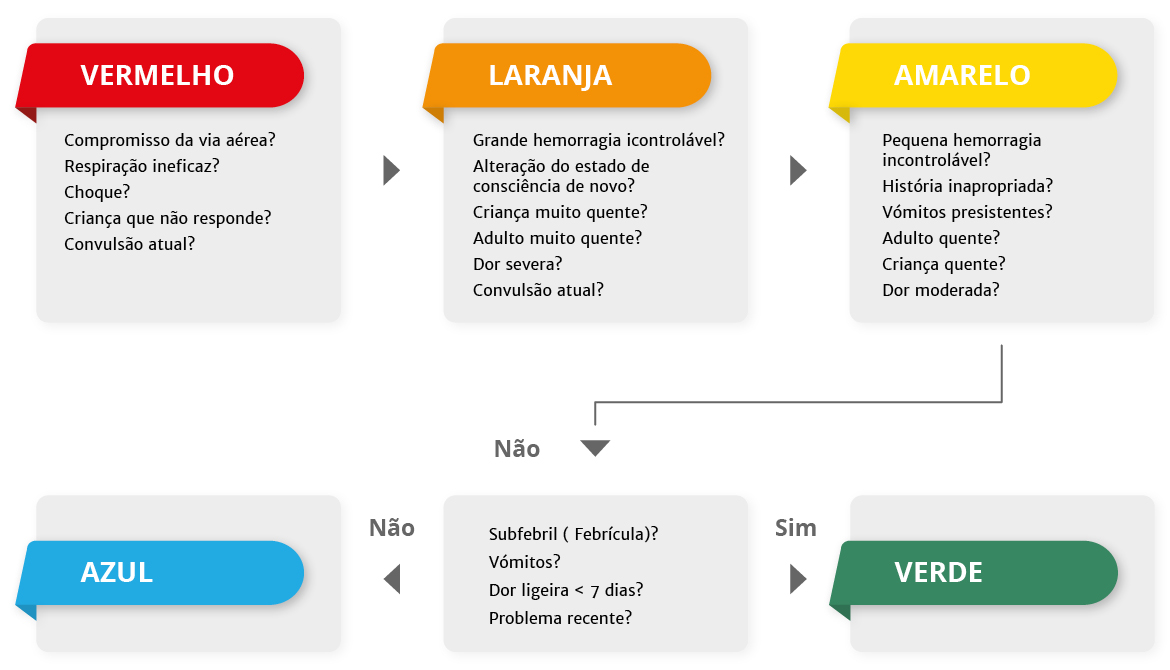
\includegraphics[width=0.9\linewidth]{img/Codigo-Cores-Atendimento-Sistema-Triagem-Manchester.jpg}  % largura percentual 
	\caption{Fluxograma da Triagem de Manchester}
	\label{fig:ccasTriagenManchester}
\end{figure}



\subsection{Testes unitários}


texto para Testes unitários...
 
\colorbox{red}{\Large falta desenvolver mais...}


\subsection{Teste do API: Swagger}


texto para Teste do API: Swagger...
 
\colorbox{red}{\Large falta desenvolver mais...}


\subsection{Teste do API: Postman}


texto para Teste do API: Postman...
 
\colorbox{red}{\Large falta desenvolver mais...}



\subsection{Documentação do API}


texto para Documentação do API...
 
\colorbox{red}{\Large falta desenvolver mais...}



% reuniões

\chapter{Milestone vAlfa: Reuniões}





\section{Reunião MA01}\label{reuniaoMA01}

\subsection*{Data:}
16-março-2022

\subsection*{Intervenientes:}
Grupo de trabalho

\subsection*{Âmbito:}
Definição do trabalho a ser realizado.

\subsection*{Descrição:}
Escolha das tasks a serem realizadas na sprint1. \\

Ficou decidido também que o colega Augusto Pereira irá continuar a desenvolver os mockups para se preparar o interface do front-end. \\


\textbf{Tasks para a sprint1}

\begin{itemize}
	\item Preparar base do projeto
	\item Testar código C\#
	\item Testar BD
	\item Preparar BD
	\item ID28-Sysadmin-criar/modificar lista de cores de triagem
	\item ID27-Sysadmin-criar/modificar lista de nacionalidades
	\item ID26-Sysadmin-adicionar/modificar/desativar utilizadores do sistema
	\item ID24-Sysadmin-criar/modificar lista de locais
	\item ID23-Sysadmin-criar/modificar lista de idiomas
	\item Fazer testes
	\item Documentação, manter atualização
\end{itemize}


\noindent \rule{\linewidth}{0.4pt}
\newline

\section{Reunião MA02}\label{reuniaoMA02}

\subsection*{Data:}
23-março-2022

\subsection*{Intervenientes:}
Grupo de trabalho e professor

\subsection*{Âmbito:}
Revisão do diagrama de classes.

Discussão sobre a abordagem a ser tomada em relação ao API.

\textbf{Diagrama de Classes}
Remover a classe "episodioQuestionario".


\textbf{API:}
Não deve ser usado EntityFrameWork para que haja controlo de todas as operações realizadas.

O API deve retornar objetos em json.

\noindent \rule{\linewidth}{0.4pt}
\newline

\section{Reunião MA03}\label{reuniaoMA03}

\subsection*{Data:}
23-março-2022

\subsection*{Intervenientes:}
Grupo de trabalho

\subsection*{Âmbito:}
Organização da trabalho da sprint; 

Discussão sobre a abordagem a ser tomada em relação ao API.


\textbf{Items para a sprint2}


\begin{itemize}
	\item Testar código C\#
	\item (API)ID28-Sysadmin-criar/modificar lista de cores de triagem
	\item (API)ID27-Sysadmin-criar/modificar lista de nacionalidades
	\item (API)ID26-Sysadmin-adicionar/modificar/desativar utilizadores do sistema
	\item (API)ID24-Sysadmin-criar/modificar lista de locais
	\item (API)ID23-Sysadmin-criar/modificar lista de idiomas
	\item (LIB)ID26-Sysadmin-adicionar/modificar/desativar utilizadores do sistema
	\item (LIB)ID28-Sysadmin-criar/modificar lista de cores de triagem
	\item (LIB)ID27-Sysadmin-criar/modificar lista de nacionalidades
	\item (LIB)ID24-Sysadmin-criar/modificar lista de locais
	\item (LIB)ID23-Sysadmin-criar/modificar lista de idiomas
	\item Fazer testes (console, gerador de ID único)
	\item Melhorar mockups
	\item Documentação, manter atualização
\end{itemize}

\noindent \rule{\linewidth}{0.4pt}
\newline

\section{Reunião MA04}\label{reuniaoMA04}

\subsection*{Data:}
30-março-2022

\subsection*{Intervenientes:}
Grupo de trabalho

\subsection*{Âmbito:}
Revisão do trabalho realizado na sprint.

\noindent \rule{\linewidth}{0.4pt}
\newline

\section{Reunião MA05}\label{reuniaoMA05}

\subsection*{Data:}
30-março-2022

\subsection*{Intervenientes:}
Grupo de trabalho

\subsection*{Âmbito:}
Planeamento do trabalho a ser realizado na sprint.

\textbf{Items para a sprint3}

\begin{itemize}
	\item (LIB) DB thread safe access
	\item (LIB) ORM design+implementation
	\item Testar código C\#
	\item UnitTests (new project to solution)
	\item (API)ID28-Sysadmin-criar/modificar lista de cores de triagem
	\item (API)ID27-Sysadmin-criar/modificar lista de nacionalidades
	\item (API)ID26-Sysadmin-adicionar/modificar/desativar utilizadores do sistema
	\item (API)ID24-Sysadmin-criar/modificar lista de locais
	\item (API)ID23-Sysadmin-criar/modificar lista de idiomas
	\item Documentação, manter atualização
\end{itemize}

\noindent \rule{\linewidth}{0.4pt}
\newline

\section{Reunião MA06}\label{reuniaoMA06}

\subsection*{Data:}
06-abril-2022

\subsection*{Intervenientes:}
Grupo de trabalho e professor

\subsection*{Âmbito:}
Revisão do trabalho realizado nas duas ultimas sprints. 

Discussão e validação dos testes unitários utilizados. 

Discussão acerca de ferramentas úteis para testes do API.

\noindent \rule{\linewidth}{0.4pt}
\newline
\section{Reunião MA07}\label{reuniaoMA07}

\subsection*{Data:}
7-abril-2022

\subsection*{Intervenientes:}
Grupo de trabalho

\subsection*{Âmbito:}

\textbf{Items para a sprint4}

\begin{itemize}
	\item (API)ID28-Sysadmin-criar/modificar lista de cores de triagem
	\item (API)ID27-Sysadmin-criar/modificar lista de nacionalidades
	\item (API)ID26-Sysadmin-adicionar/modificar/desativar utilizadores do sistema
	\item (API)ID24-Sysadmin-criar/modificar lista de locais
	\item (API)ID23-Sysadmin-criar/modificar lista de idiomas
	\item Utilizador(generico) autenticar
	\item (API)ID9-Triagem - associar um utente ao episodio 
	\item (API)ID8-Triagem - criar episodios
	\item Documentação, manter atualização
	\item (LIB)Criação de camada DAL
	\item (API)ID16-Utente - consultar os meus dados
	\item (API)ID17-Utente - corrigir/alterar resposta questionario
	\item (API)ID29-Utente - Obter Lista de Questionario
	\item Criar Teste para o API
	\item (API)ID6-Enfermeiro-saber a localização de um utente
	\item (API)ID7-Medico-saber a localização de um utente
	\item (API)ID4-Utilizador-saber a localização
	\item (API)ID4-Acompanhante-saber a localização do utente que acompanha
	\item (LIB)ID23-Sysadmin-criar/modificar lista de idiomas
	\item (LIB)ID24-Sysadmin-criar/modificar lista de locais
	\item (LIB)ID27-Sysadmin-criar/modificar lista de nacionalidades
	\item (API)ID25-Sysadmin-criar/modificar lista de tipos de dados métricos
	\item (LIB)ID25-Sysadmin-criar/modificar lista de tipos de dados métricos
	\item (LIB) testes unitários, código e dados para testes
	\item (API)implementar '/OSLER/Lista/*' listas de apoio para o front-end
	\item (API)Sysadmin-criar/modificar lista de itensFluxoManchester
	\item (LIB)Sysadmin-criar/modificar lista de itensFluxoManchester
	\item (LIB)PlayLib, verificar/criar/inicializar tabelas na BD
\end{itemize}


\noindent \rule{\linewidth}{0.4pt}
\newline
\section{Reunião MA08}\label{reuniaoMA08}

\subsection*{Data:}
14-abril-2022

\subsection*{Intervenientes:}
Grupo de trabalho

\subsection*{Âmbito:}
Revisão do trabalho realizado nas ultima sprint. 

Escolha do Plataforma Postman para suportar testes à API. 

Criação da equipa no Postman.


\noindent \rule{\linewidth}{0.4pt}
\newline
\section{Reunião MA09}\label{reuniaoMA09}

\subsection*{Data:}
14-abril-2022

\subsection*{Intervenientes:}
Grupo de trabalho

\subsection*{Âmbito:}

\textbf{Items para a sprint5}

\begin{itemize}
	\item (API)ID8-Triagem - criar episodios
	\item (API)ID16-Utente - consultar os meus dados
	\item (API)ID17-Utente - corrigir/alterar resposta questionario
	\item (API)ID29-Utente - Obter Lista de Questionario
	\item (API)ID22-Sysadmin-criar/modificar lista de questionários
	\item (API)ID1-Utilizador(generico)-autenticar
	\item (API)ID3-Acompanhante-responder a questionarios sobre o utente
	\item (API)ID18-Enfermeiro-consultar os dados de um utente
	\item (API)ID2-Utente-responder a questionarios 
	\item (API)ID10-Utilizador(generico)-introduzir dados metricos relativos ao paciente
	\item (API)ID11-Utilizador(generico)-visualizar os seus dados metricos
	\item (API)ID5-Acompanhante-saber a localização do utente que acompanha
	\item (API)ID6-Enfermeiro-saber a localização de um utente
	\item (API)ID30-Medico-alterar a localização de um utente
	\item (API)ID20-Medico-alterar o estado de um episodio
	\item (API)ID21-Medico-chamar pelo utente, alterando a sua localização
	\item (API)ID19-Medico-consultar episodios anteriores do utente (historico)
	\item (API)ID7-Medico-saber a localização de um utente
	\item (API)ID15-Medico-saber as respostas dadas pelo utente e acompanhante
	\item (API)ID4-Utente-saber a localização
	\item Documentação, manter atualização
	\item (LIB) LoginRegisto+LoginRegistoDao
	\item (LIB) Questionario+QuestionarioDao
	\item (LIB) EpisodioHistLocal+EpisodioHistLocalDao
	\item (LIB) EpisodioQuestionario
	\item (LIB) EpisodioRegistoDados
	\item (LIB) Pergunta+PerguntaDao
	\item (LIB) EpisodioNotificacaoDao
\end{itemize}

\noindent \rule{\linewidth}{0.4pt}
\newline

\section{Reunião MA10}\label{reuniaoMA10}

\subsection*{Data:}
20-abril-2022

\subsection*{Intervenientes:}
Grupo de trabalho e professor

\subsection*{Âmbito:}
Revisão do trabalho realizado nas duas ultimas sprints. 

Revisão dos testes realizados e a formulação dos mesmos. 

Discussão acerca de bugs conhecidos do Swagger e formas de ultrapassa-los. 

Recomendação e escolha do Swagger Examples para testes da API.

\noindent \rule{\linewidth}{0.4pt}
\newline
\section{Reunião MA11}\label{reuniaoMA11}

\subsection*{Data:}
20-abril-2022

\subsection*{Intervenientes:}
Grupo de trabalho e professor

\subsection*{Âmbito:}

\textbf{Items para a sprint6}

\begin{itemize}
	\item (API)- Swagger- completar exemplos de teste
	\item (API)ID16-Utente - consultar os meus dados
	\item (API)ID17-Utente - corrigir/alterar resposta questionario
	\item (API)ID3-Acompanhante-responder a questionarios sobre o utente
	\item (API)ID15-Medico-saber as respostas dadas pelo utente e acompanhante
	\item Documentação, manter atualização
	\item Verificação do código C\# (LIB+API)
	\item (API)ID1-Utilizador(generico)-autenticar
	\item (API)ID18-Enfermeiro-consultar os dados de um utente
	\item (API)ID20-Medico-alterar o estado de um episodio
	\item (API)ID19-Medico-consultar episodios anteriores do utente (historico)
	\item (API)ID12-Sysadmin-repor a palavra-passe de um enfermeiro
	\item (API)ID13-Sysadmin-repor a palavra-passe de um medico
	\item (API)ID14-Sysadmin-repor a palavra-passe de um utilizador de triagem
	\item (LIB)ORM-Testar e/ou corrigir acesso paralelo + singleton
	\item (API)ID31-Utente-Login/Autenticar no Episodio
	\item (API)ID32-Acompanhante-Login/Autenticar no Episodio
	\item (LIB)Validar login e registar histórico
	\item (LIB)ID19-Medico-consultar episodios anteriores do utente (historico)
	\item (LIB)ID31-Utente-Login/Autenticar no Episodio
	\item (LIB)ID32-Acompanhante-Login/Autenticar no Episodio
	\item (LIB)PlayLib, verificar/criar/inicializar episódios teste na BD
\end{itemize}

\noindent \rule{\linewidth}{0.4pt}
\newline
\section{Reunião MA12}\label{reuniaoMA12}

\subsection*{Data:}
27-abril-2022

\subsection*{Intervenientes:}
Grupo de trabalho e professor

\subsection*{Âmbito:}
Revisão do trabalho realizado nas duas ultimas sprints. 

Revisão do trabalho realizado ao longo da millestone.

Ponderação sobre o trabalho realizado e o adiamento ou não da fim da milestone.

Adiamento do fim da milestone uma semana, para que sejam concluídos alguns detalhes da fase Alpha.

Documentar os bugs identificados.

Revisão do diagrama de classes com pormenor.

Debate sobre a gestão de acesso à aplicação.

\noindent \rule{\linewidth}{0.4pt}
\newline
\section{Reunião MA13}\label{reuniaoMA13}

\subsection*{Data:}
27-abril-2022

\subsection*{Intervenientes:}
Grupo de trabalho e professor

\subsection*{Âmbito:}

\textbf{Tasks:}

\begin{itemize}
	\item (API)ID17-Utente - corrigir/alterar resposta questionario
	\item Documentação, manter atualização
	\item Verificação do código C\# (LIB+API)
	\item Postman-Atualizar testes
	\item Swagger-Atualizar documentação/testes
	\item UnitTests-Completar com mais cenários
	\item Verificar e corrigir a estrutura de alguns controladores( medico)
	
\end{itemize}


\noindent \rule{\linewidth}{0.4pt}
\newline
\section{Reunião MA14}\label{reuniaoMA14}

\subsection*{Data:}
4-maio-2022

\subsection*{Intervenientes:}
Grupo de trabalho e professor

\subsection*{Âmbito:}
Revisão do trabalho realizado na ultima sprint. 

Revisão do trabalho realizado ao longo da millestone.



\noindent \rule{\linewidth}{0.4pt}
\newline
% Milestone vBeta

\chapter{Milestone vBeta}

texto para Milestone vBeta...


\subsection{Tasks vBeta}

\begin{itemize}
	\item Tasks Sprint1 - Milestone vBeta;
	\item Tasks Sprint2 - Milestone vBeta;
	\item Tasks Sprint3 - Milestone vBeta;
\end{itemize}


\section{Sub-capitulo 2}
Texto do sub-capitulo 2

% reuniões

\chapter{Milestone vBeta: Reuniões}

espaço para Milestone vBeta: Reuniões...


\section{Reunião MB01}\label{reuniaoMB01}

\subsection*{Data:}
4-maio-2022

\subsection*{Intervenientes:}
Grupo de trabalho 

\subsection*{Âmbito:}
Planeamento da sprint.

Debate sobre a forma como conduzir o milestone. 

\textbf{tasks:}

\begin{itemize}
	\item elaborar uma lista de aspetos a melhorar, bugs conhecidos,
	\item postman workflow
	\item atualizar a lista os endpoints
\end{itemize}

\noindent \rule{\linewidth}{0.4pt}
\newline



% Milestone vRTW

\chapter{Milestone vRTW}

texto para Milestone vRTW...


\subsection{Tasks vRTW}

\begin{itemize}
	\item Tasks Sprint1 - Milestone vRTW.
	\item Tasks Sprint2 - Milestone vRTW.
\end{itemize}


\section{Sub-capitulo 2}
Texto do sub-capitulo 2

% reuniões

\chapter{Milestone vRTW: Reuniões}

espaço para Milestone vRTW: Reuniões...



% ?

\chapter{Capitulo 700}

Capitulo 700...


\section{Sub-capitulo 1}
Texto do sub-capitulo 1

\section{Sub-capitulo 2}
Texto do sub-capitulo 2


% ?

\chapter{Capitulo 800}

Capitulo 800...


\section{Sub-capitulo 1}
Texto do sub-capitulo 1

\section{Sub-capitulo 2}
Texto do sub-capitulo 2


% ?

\chapter{Capitulo 900}

Capitulo 900...


\section{Sub-capitulo 1}
Texto do sub-capitulo 1

\section{Sub-capitulo 2}
Texto do sub-capitulo 2



% comentar se nao tiver figuras
\listoffigures
\addcontentsline{toc}{chapter}{Lista de Figuras}

% comentar se nao tiver tabelas
%\addcontentsline{toc}{chapter}{Lista de Tabelas}
%\listoftables

% comentar se nao se quiser lista de listagens
\lstlistoflistings
\addcontentsline{toc}{chapter}{Lista de Código}

% Commentar proximas duas linhas se nao for para usar acronimos
\printglossary[type=\acronymtype,title={Siglas \& Acrónimos},toctitle={Siglas \& Acrónimos}]

% Commentar proximas duas linhas se nao for para usar glossarios
\printglossary[title={Indice de Termos},toctitle={Indice de Termos}]

% comentar se não for para usar bibliografia
\bibliography{biblio}
\addcontentsline{toc}{chapter}{Bibliografia}

\end{document} 
